\section{硬件设计}

\subsection{电源系统总体设计}

空中机器人以标称\qty{48}{\V}电源作为一次母线。考虑到后级降压模块输入端配置有较大的储能电容，若电池直接接入，电容近似短路会产生较大的瞬态冲击电流，并在连接器处形成电弧。为此，我们在一次母线入口设置\qty{48}{\V}电源缓启动模块，使母线电压以受控斜率建立；缓启动后的\qty{48}{\V}母线进入两级同步Buck变换器，先降压至\qty{24}{\V}，再由\qty{24}{\V}降压至\qty{12}{\V}，从而为无人机上不同电压等级的负载供电。电源树可概括为：

\[
\qty{48}{\V}\text{电源}
\longrightarrow
\qty{48}{\V}\text{缓启动}
\longrightarrow
\qty{48}{\V}\!\rightarrow\!\qty{24}{\V}\text{同步降压}
\longrightarrow
\qty{24}{\V}\!\rightarrow\!\qty{12}{\V}\text{同步降压}
\]

三个模块均在输入、输出端设置瞬态抑制与分布式去耦，并通过低阻抗功率器件、并联MOSFET和大面积功率回路降低导通损耗。各模块的主要设计参数如\tabref{tab:drone_power_tree_parameters}所示。

\begin{table}[hbtp!]
    \centering
    \begin{tabular}{m{2.7cm} m{2.8cm} m{3.5cm} m{5.0cm}}
    \toprule
    模块 & 输入/输出 & 核心器件或拓扑 & 原理图关键参数 \\
    \midrule
    \qty{48}{\V}电源缓启动
    & \qty{48}{\V}/\qty{48}{\V}
    & LM5069-2热插拔控制器、四管并联高侧开关
    & 两颗\qty{470}{\micro\farad}母线电容，输入/输出SMBJ54A瞬态抑制二极管 \\
    \midrule
    \qty{48}{\V}转\qty{24}{\V}
    & \qty{48}{\V}/\qty{24}{\V}
    & MP9931同步Buck控制器、上下桥臂各两管并联
    & \qty{22}{\micro\henry}电感，\qty{3}{\milli\ohm}电流采样电阻，\qty{220}{\kilo\ohm}/\qty{7.5}{\kilo\ohm}反馈分压 \\
    \midrule
    \qty{24}{\V}转\qty{12}{\V}
    & \qty{24}{\V}/\qty{12}{\V}
    & MP9931同步Buck控制器、上下桥臂各两管并联
    & \qty{15}{\micro\henry}电感，\qty{2}{\milli\ohm}电流采样电阻，\qty{160}{\kilo\ohm}/\qty{11.5}{\kilo\ohm}反馈分压 \\
    \bottomrule
    \end{tabular}
    \caption{无人机电源树主要设计参数}
    \label{tab:drone_power_tree_parameters}
\end{table}

\subsection{48V电源缓启动模块}

\begin{figure}[hbtp!]
    \centering
    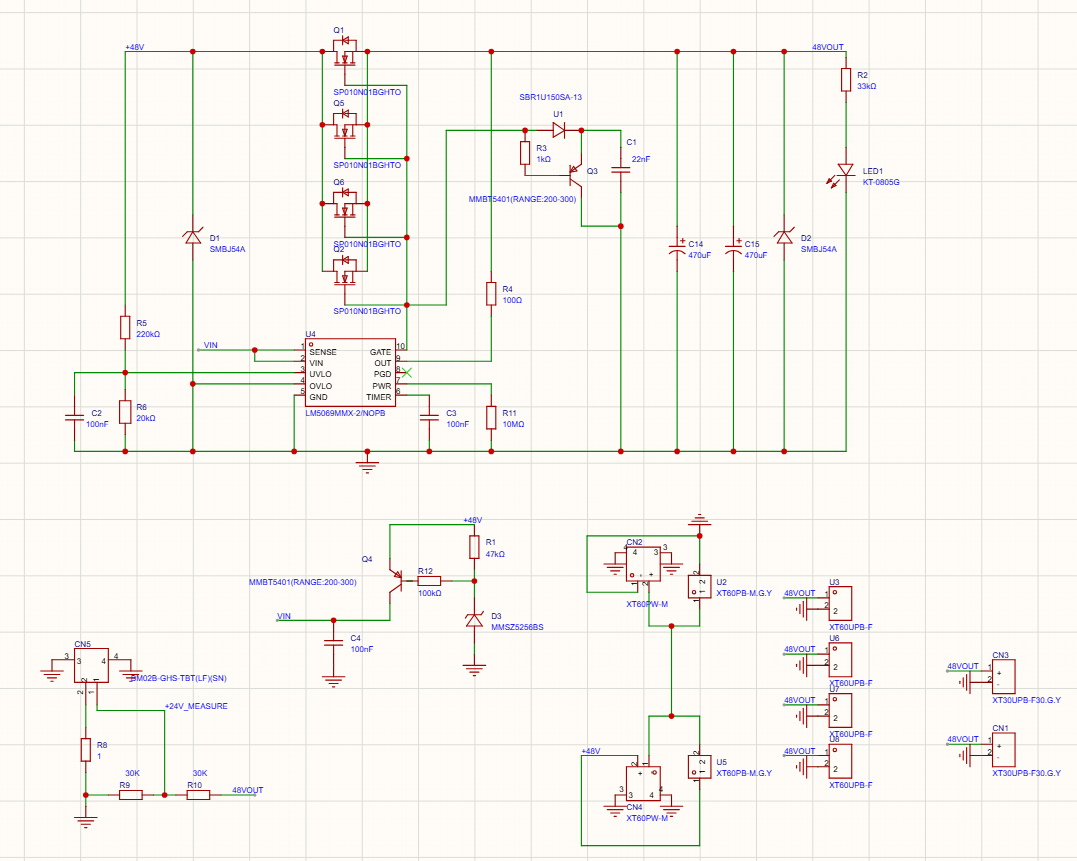
\includegraphics[width=0.95\columnwidth]{figure/4_详细设计/硬件设计/48V电源缓启动原理图.png}
    \caption{48V电源缓启动模块原理图}
    \label{fig:48v_soft_start_schematic}
\end{figure}

缓启动模块的原理图如\figref{fig:48v_soft_start_schematic}所示。模块采用LM5069-2作为高压热插拔及浪涌电流控制器。该器件适用于\qty{9}{\V}至\qty{80}{\V}正电源系统，可驱动外置N沟道MOSFET，并具备欠压锁定、过压锁定、故障定时和自动重启功能。相比使用功率电阻串联后再旁路的方案，MOSFET线性缓启动没有机械触点，启动过程可重复，且稳态导通损耗更低。

主功率通路由四颗\qty{100}{\V}等级N沟道MOSFET并联构成。并联连接能够减小等效导通电阻并分担稳态电流；布局时需要保证四条支路的漏极、源极铜皮和栅极驱动路径近似对称，避免寄生电阻与寄生电感差异造成静态及动态电流分配不均。LM5069-2的GATE端控制MOSFET栅极电压，外围三极管、二极管与\qty{22}{\nano\farad}电容组成栅极斜率控制网络，使输出电压按设定的$\mathrm{d}V/\mathrm{d}t$上升。启动阶段的电容充电电流近似为

\begin{equation}
    I_{\mathrm{inrush}} \approx C_{\mathrm{out}}\frac{\mathrm{d}V_{\mathrm{out}}}{\mathrm{d}t} ,
    \label{equ:soft_start_inrush_current}
\end{equation}

因此减小输出电压上升斜率即可限制浪涌电流。原理图中两颗\qty{470}{\micro\farad}电解电容并联，得到约\qty{940}{\micro\farad}的母线储能电容；其在\qty{48}{\V}下储存的能量为

\begin{equation}
    E_{\mathrm{bus}}=\frac{1}{2}C_{\mathrm{out}}V_{\mathrm{out}}^2
    \approx \frac{1}{2}\times\qty{940}{\micro\farad}\times(\qty{48}{\V})^2
    \approx\qty{1.08}{\joule}
    \label{equ:48v_bus_capacitor_energy}
\end{equation}

该能量若在插接瞬间释放，将对连接器和前级电源产生明显冲击，说明设置缓启动模块是必要的。R5与R6构成欠压检测分压网络；按LM5069典型\qty{2.5}{\V}比较阈值估算，其静态开启门限约为

\begin{equation}
    V_{\mathrm{UVLO}} \approx \qty{2.5}{\V}
    \left(1+\frac{\qty{220}{\kilo\ohm}}{\qty{20}{\kilo\ohm}}\right)
    \approx\qty{30}{\V}
    \label{equ:48v_uvlo_threshold}
\end{equation}

实际门限还会受到芯片迟滞电流与电阻容差影响。输入端和输出端分别设置SMBJ54A瞬态抑制二极管，用于吸收插拔及长线缆寄生电感引起的尖峰；电源指示、母线电压采样和多组XT60/XT30接口则用于状态确认及后级配电。设计验证时需要重点检查MOSFET在线性区启动时的安全工作区、最不利输入电压下的启动时间，以及短路或重复重启条件下的结温累积。

\subsection{48V转24V降压模块}

\begin{figure}[hbtp!]
    \centering
    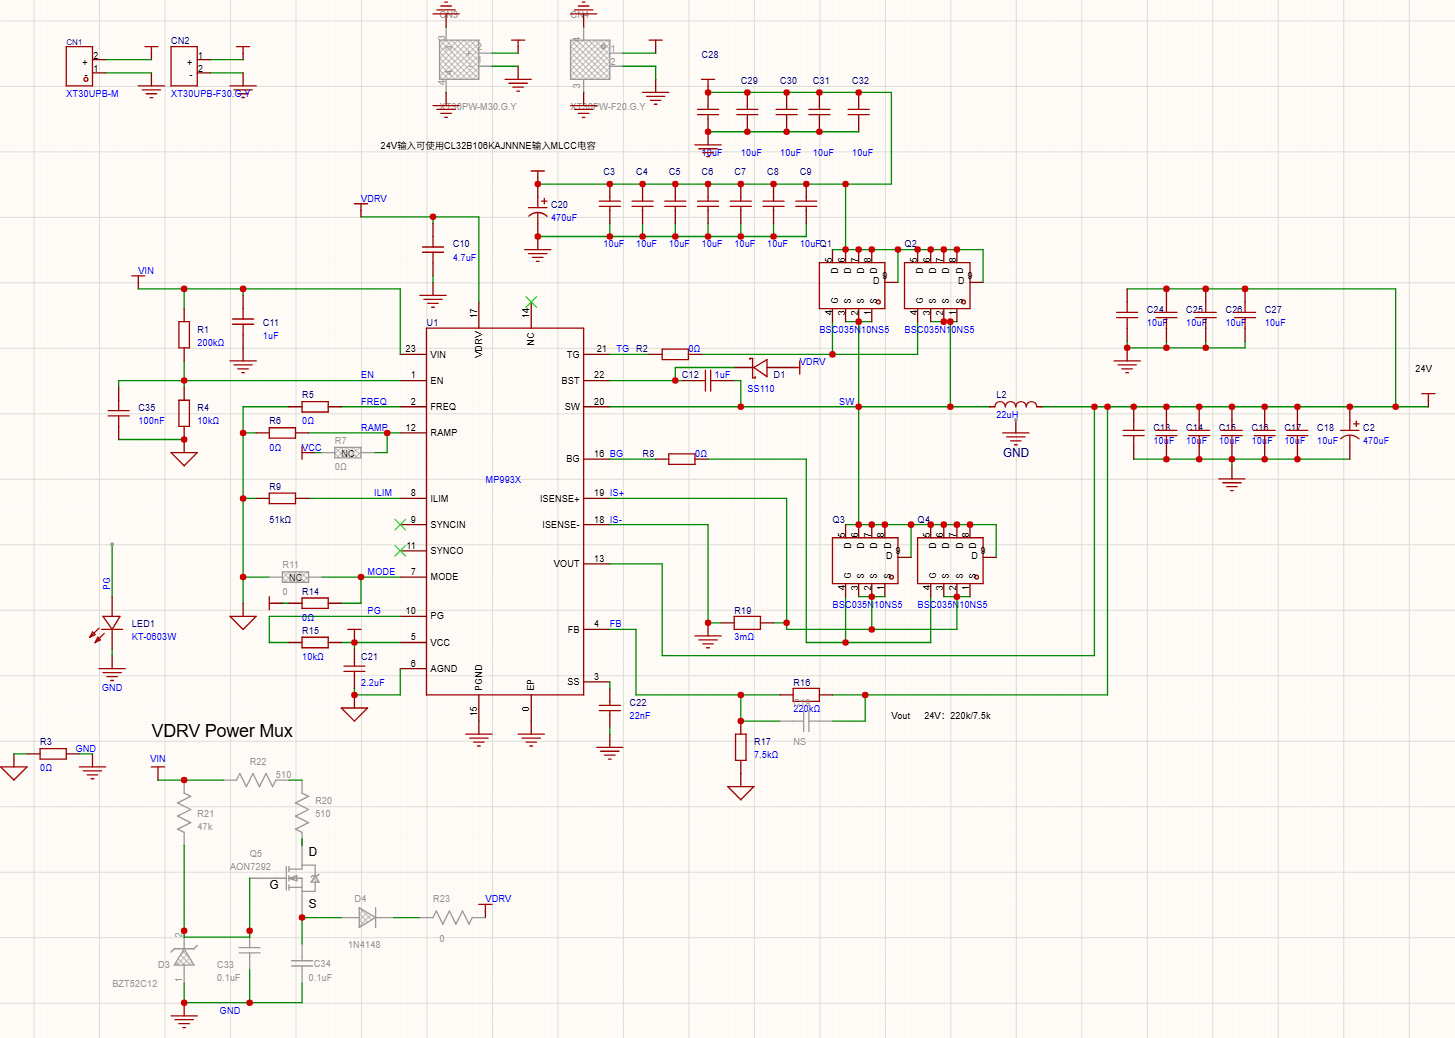
\includegraphics[width=0.98\columnwidth]{figure/4_详细设计/硬件设计/48V转24V降压模块原理图.png}
    \caption{48V转24V同步降压模块原理图}
    \label{fig:48v_to_24v_buck_schematic}
\end{figure}

\qty{48}{\V}转\qty{24}{\V}模块的原理图如\figref{fig:48v_to_24v_buck_schematic}所示。控制器采用MP9931高压同步Buck控制器。该器件的输入电压范围覆盖无人机\qty{48}{\V}母线，采用恒定导通时间控制，能够直接驱动上下桥臂N沟道MOSFET，并通过FREQ、RAMP、ILIM与MODE等引脚配置开关频率、斜坡补偿、电流限制和轻载工作方式。

功率级上下桥臂均采用两颗BSC035N10NS5并联。该MOSFET的耐压为\qty{100}{\V}，在\qty{10}{\V}栅极驱动下最大导通电阻为\qty{3.5}{\milli\ohm}；两颗并联后，单个桥臂的室温等效导通电阻理论值约为\qty{1.75}{\milli\ohm}。相较单管方案，并联结构可降低大电流条件下的$I^2R$损耗并分散热源。桥臂中点经\qty{22}{\micro\henry}功率电感与输出电容阵列滤波后形成\qty{24}{\V}母线，\qty{3}{\milli\ohm}分流电阻向控制器提供电流检测信号。输入、输出端均采用大容量电解电容与多颗MLCC并联，以分别承担低频负载阶跃和高频开关纹波。

MP9931反馈基准电压为\qty{0.8}{\V}，输出电压由上、下反馈电阻决定：

\begin{equation}
    V_{\mathrm{out}}=V_{\mathrm{FB}}
    \left(1+\frac{R_{\mathrm{top}}}{R_{\mathrm{bottom}}}\right)
    \label{equ:mp9931_feedback_voltage}
\end{equation}

代入原理图中的$R_{\mathrm{top}}=\qty{220}{\kilo\ohm}$、$R_{\mathrm{bottom}}=\qty{7.5}{\kilo\ohm}$，可得

\begin{equation}
    V_{\mathrm{out}}
    =\qty{0.8}{\V}\left(1+\frac{220}{7.5}\right)
    \approx\qty{24.27}{\V}
    \label{equ:48v_to_24v_feedback}
\end{equation}

与\qty{24}{\V}母线的目标值一致。在标称输入电压下，理想占空比约为$D=V_{\mathrm{out}}/V_{\mathrm{in}}\approx0.5$。电感纹波电流可由

\begin{equation}
    \Delta I_L=\frac{(V_{\mathrm{in}}-V_{\mathrm{out}})D}{L f_{\mathrm{sw}}}
    \label{equ:buck_inductor_ripple}
\end{equation}

进行校核，并结合电感饱和电流、MOSFET结温和输出纹波确定最终开关频率。VDRV Power Mux网络为栅极驱动电源提供钳位与隔离；当输出建立后，由较低电压侧为驱动电路供电，可减小控制器内部高压偏置电路的功耗。该模块PCB设计中应将输入电容、上下桥臂MOSFET与功率地构成的高频换流环路尽可能缩短，并将反馈走线与开关节点隔离。

\subsection{24V转12V降压模块}

\begin{figure}[hbtp!]
    \centering
    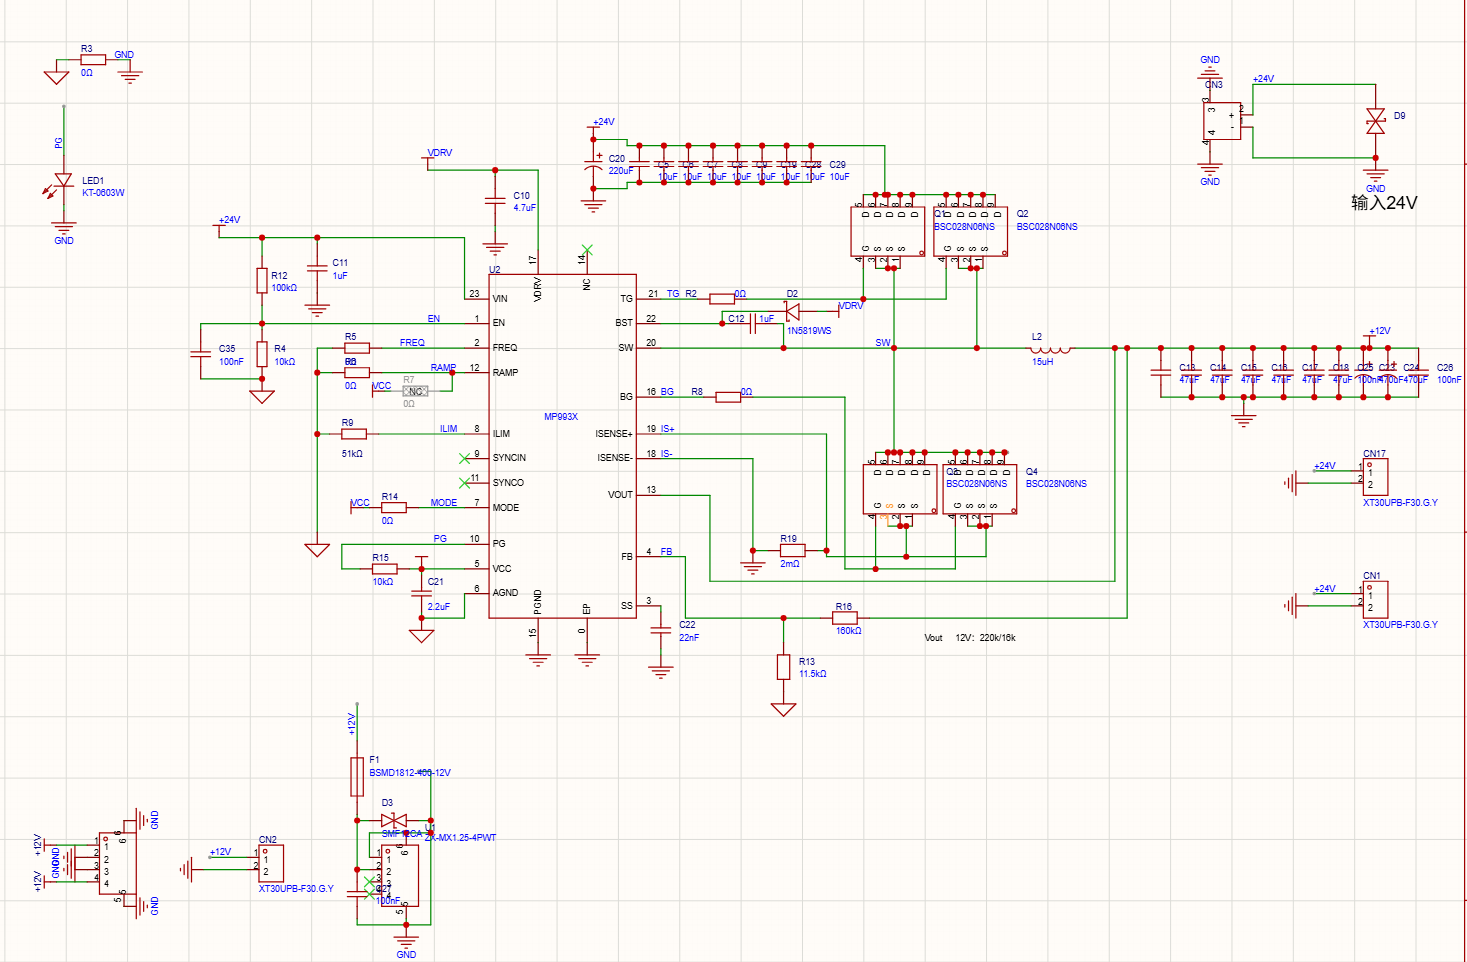
\includegraphics[width=0.98\columnwidth]{figure/4_详细设计/硬件设计/24V转12V降压模块原理图.png}
    \caption{24V转12V同步降压模块原理图}
    \label{fig:24v_to_12v_buck_schematic}
\end{figure}

\qty{24}{\V}转\qty{12}{\V}模块的控制结构与前级保持一致，如\figref{fig:24v_to_12v_buck_schematic}所示。复用MP9931控制器及同步Buck拓扑可以减少器件种类和调试工作量，同时保留欠压、过流和过温等保护能力。由于本级输入电压降低，功率级MOSFET选用\qty{60}{\V}耐压的BSC028N06NS；其在\qty{10}{\V}栅极驱动下最大导通电阻为\qty{2.8}{\milli\ohm}，每个桥臂两管并联后的理论等效导通电阻约为\qty{1.4}{\milli\ohm}。本级采用\qty{15}{\micro\henry}功率电感和\qty{2}{\milli\ohm}电流采样电阻，以适配较低输出电压下的纹波及电流检测需求。

反馈网络使用$R_{\mathrm{top}}=\qty{160}{\kilo\ohm}$和$R_{\mathrm{bottom}}=\qty{11.5}{\kilo\ohm}$。由\eqref{equ:mp9931_feedback_voltage}可得

\begin{equation}
    V_{\mathrm{out}}
    =\qty{0.8}{\V}\left(1+\frac{160}{11.5}\right)
    \approx\qty{11.93}{\V}
    \label{equ:24v_to_12v_feedback}
\end{equation}

满足\qty{12}{\V}负载的供电需求；在标称工况下，本级理想占空比同样约为0.5。输出端使用多颗\qty{47}{\micro\farad}MLCC、\qty{470}{\micro\farad}电解电容与\qty{100}{\nano\farad}高频去耦电容组成宽频段滤波网络，并在配电支路设置自恢复保险丝和瞬态抑制器件，降低单路负载故障向\qty{12}{\V}主母线扩散的风险。输入端的瞬态抑制二极管用于限制\qty{24}{\V}线缆及前级变换器引起的尖峰。

两级Buck模块在定型前均需完成空载启动、满载稳态、负载阶跃、输入电压扫描和短路保护测试，并记录效率、输出纹波、MOSFET及电感最高温升。上述性能参数将在样机测试完成后写入测试结果，本节暂不以理论估算代替实测结论。

\clearpage
